\documentclass[border=4pt]{standalone}
\usepackage{tikz}
\usetikzlibrary{arrows.meta}
\begin{document}
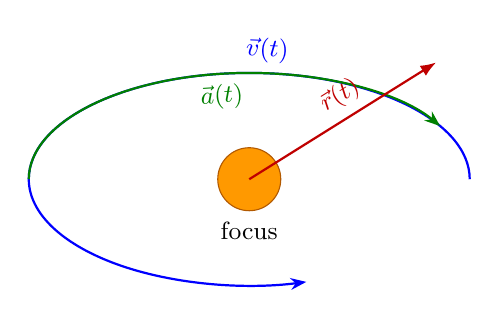
\begin{tikzpicture}[auto,orbit/.style={-{Stealth[length=2mm]},thick},every node/.append style={font=\small}]
  \fill[orange!80!yellow] (0,0) circle (4mm);
  \draw[orange!70!black] (0,0) circle (4mm);
  \node[below] at (0,-.42) {focus};

  \draw[orbit,blue] (2.8,0)
    arc[start angle=0,end angle=285,x radius=2.8cm,y radius=1.35cm]
    node[pos=.3,sloped] {$\vec v(t)$};
  \draw[orbit,green!50!black] (-2.8,0)
    arc[start angle=180,end angle=30,x radius=2.8cm,y radius=1.35cm]
    node[pos=.55,sloped,swap] {$\vec a(t)$};
  \draw[red!75!black,thick,-{Latex[length=2mm]}] (0,0) -- (32:2.8cm)
    node[pos=.55,sloped] {$\vec r(t)$};
\end{tikzpicture}
\end{document}
